\documentclass[12pt]{article}

\usepackage{sbc-template}

\usepackage{graphicx,url}

\usepackage[brazil]{babel}   
\usepackage[latin1]{inputenc}  

     
\sloppy

\title{Estruturas de dados eficientes\\ para algoritmo gen\'{e}tico}

\author{Raphael R. Gon\c{c}alves\inst{1}}


\address{Instituto de Computa\c{c}\~{a}o -- Universidade Federal Fluminense
  (UFF)\\
  24.210-346 -- Niter\'{o}i -- RJ -- Brasil
}

\begin{document} 

\maketitle

\begin{abstract}
    TODO
\end{abstract}
     
\begin{resumo} 
    A FAZER
\end{resumo}


\section{Introdu\c{c}\~{a}o}

TODO

\section{Revis\~{a}o da Literatura} \label{sec:firstpage}

TODO

\section{O Algoritmo Gen\'{e}tico}

TODO

\section{Desafios durante a implementa\c{c}\~{a}o}

TODO

\subsection{Rota\c{c}\~{a}o de vetores}

A rota\c{c}\~{a}o de vetores \'{e} uma opera\c{c}\~{a}o aplicada em \textit{arrays} e outros
\textit{containers} utilizada diferentes casos de uso na computa\c{c}\~{a}o.
Ela consiste em retirar um elemento de uma das extremidades do vetor e
inser\'{i}-lo na outra extremidade, causando a movimenta\c{c}\~{a}o de todos os elementos
para a esquerda ou para a direita, dependendo de qual a extremidade que o elemento
foi removido.

Dentro do contexto de algoritmos gen\'{e}ticos, para realizar um \textit{crossover} pode ser
necess\'{a}rio realizar diferentes opera\c{c}\~{o}es em um vetor, e uma delas que \'{e} muito
utilizada \'{e} a rota\c{c}\~{a}o. Um dos operadores de \textit{crossover} que requer uma
rota\c{c}\~{a}o \'{e} o \textit{Order Crossover} (OX), onde \'{e} selecionado um subconjunto dos genes
de um indiv\'{i}duo e inserido em outro indiv\'{i}duo, causando uma rota\c{c}\~{a}o dos elementos j\'{a}
inseridos no segundo indiv\'{i}duo tanto para a direita quanto para a esquerda. Este comportamento \'{e}
ilustrado na Figura~\ref{fig:orderCrossover}

\begin{figure}[ht]
\centering
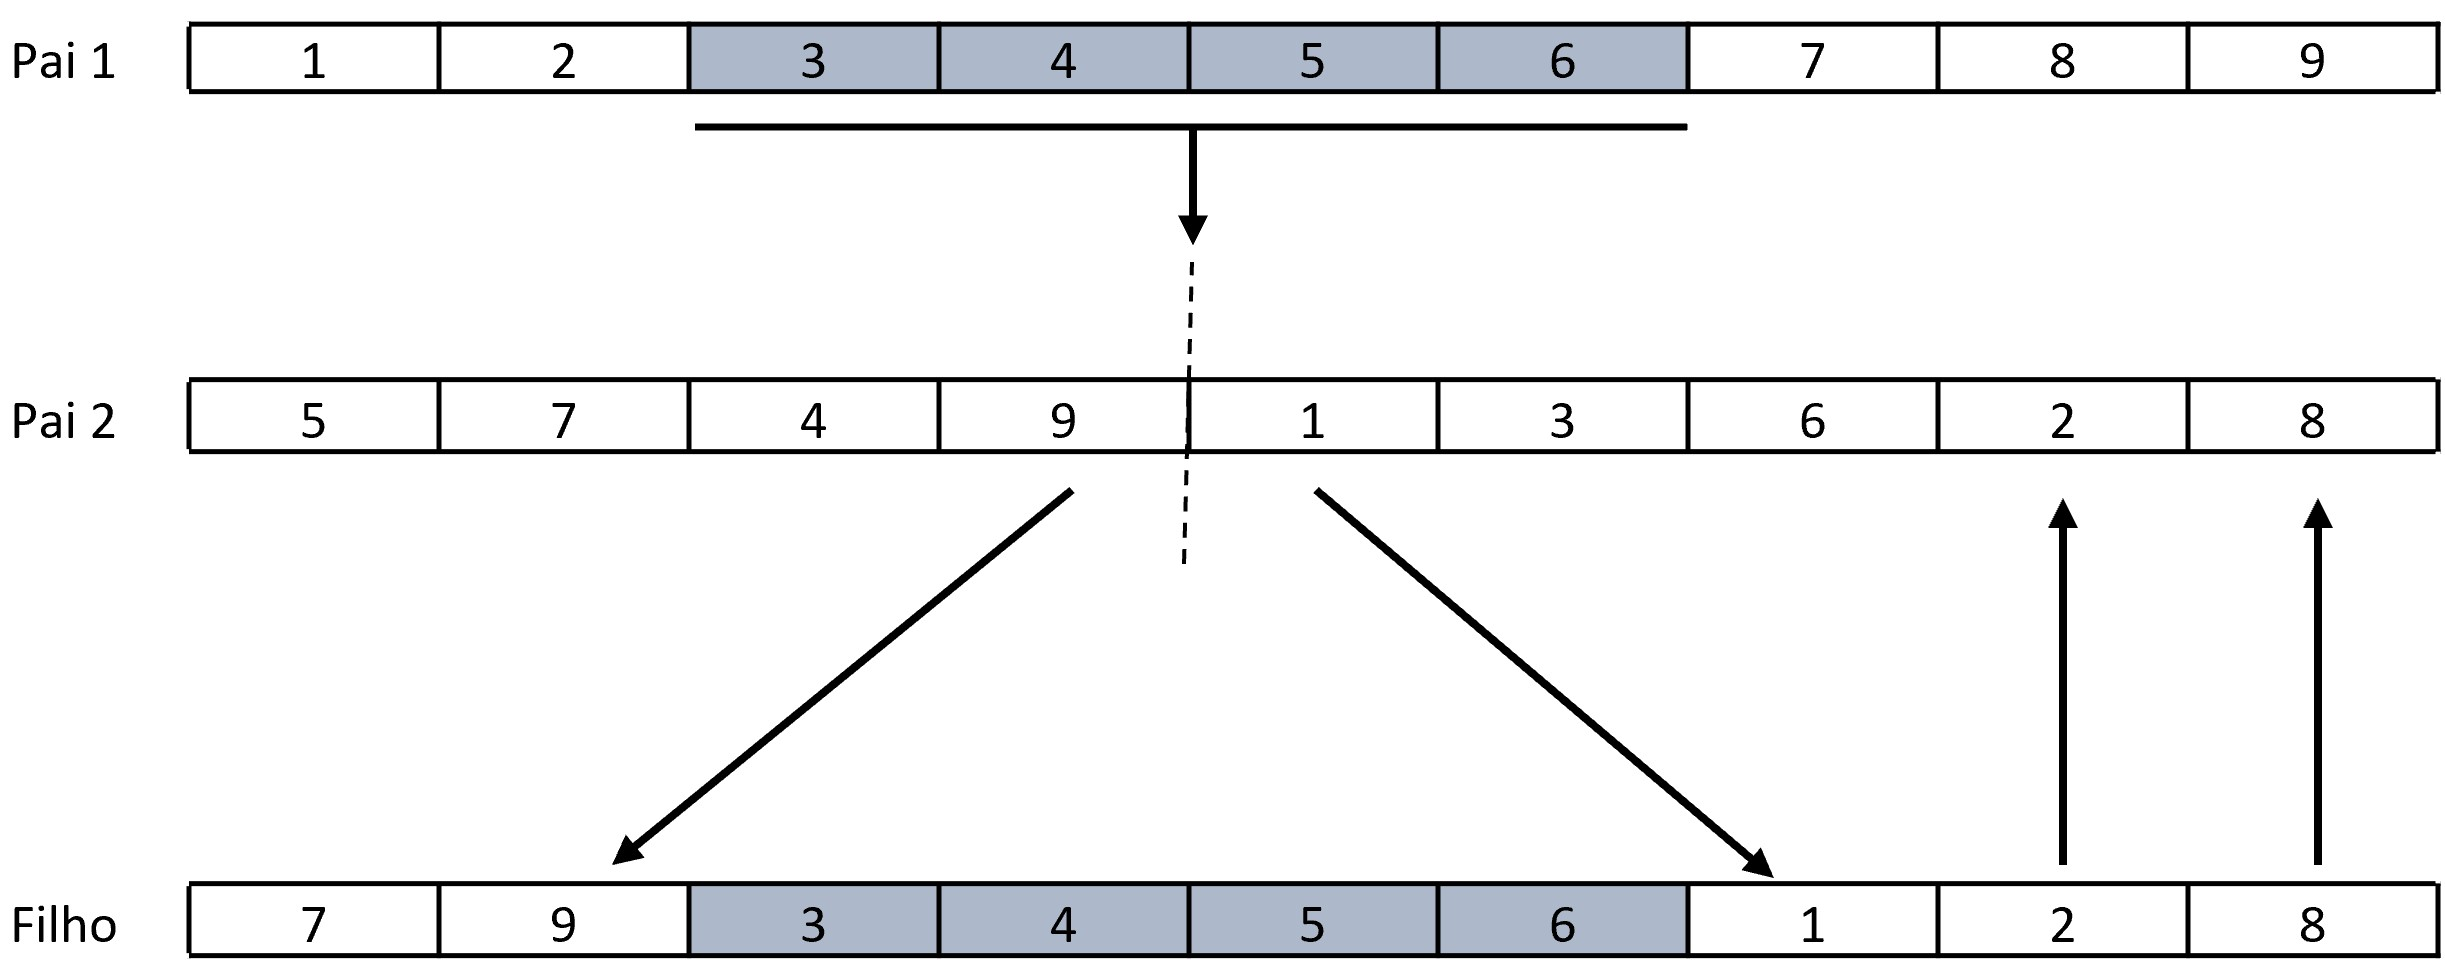
\includegraphics[width=.8\textwidth]{order_crossover.jpg}
\caption{O funcionamento do Order Crossover}
\label{fig:orderCrossover}
\end{figure}

Dependendo da estrutura de dados e o algoritmo utilizado, uma rota\c{c}\~{a}o pode levar \`{a}
copia de todos os elementos de um \textit{container} para outro, tendo em vista que, por exemplo,
um vetor somente permite a inser\c{c}\~{a}o de elementos em somente uma extremidade. Este
comportamento pode tornar esta simples tarefa uma, rotina de complexidade $\mathcal{O}(n)$.

Entretanto esta complexidade pode ser reduzida simplesmente utilizando uma estrutura do tipo
\textit{Deque} (\textit{Double-Ended Queue}). Esta estrutura de dados permite que sejam inseridos
elementos por ambos os lados, permitindo a rota\c{c}\~{a}o dos elementos com complexidade
$\mathcal{O}(1)$ com f\'{a}cil implementa\c{c}\~{a}o.

Vale ressaltar que a estrutura de \textit{hash} n\~{a}o suporta ordena\c{c}\~{a}o, ent\~{a}o
ainda \'{E} necess\'{a}rio utilizar um vetor para guardar os valores gerados. Esta decis\~{a}o
aumenta o consumo de mem\~{a}ria RAM mas pode diminuir consideravelmente o tempo de processamento.

\subsection{Gera\c{c}\~{a}o aleat\'{o}ria de elementos n\~{a}o repetitivos}\label{sec:nonRepeating}

Ao inicializar uma popula\c{c}\~{a}o de indiv\'{i}duos aleatoriamente, em muitos casos existe
a necessidade de um indiv\'{i}duo n\~{a}o possuir genes com valores repetidos. Ou seja, a cada novo
elemento inserido com um valor aleat\'{o}rio, deve-se certificar se o mesmo j\'{a} foi inserido
anteriormente. Caso positivo, devem ser gerados valores aleat\'{o}rios at\'{e} que esta
condic\c{c}\~{a}o se torne falsa, e ent\~{a}o o elemento \'{e} inserido no cromossomo do indiv\'{i}duo.

Como pode-se perceber, podem ser necess\'{a}rias muitas buscas sucessivas no vetor de genes para verificar
a exist\^{e}ncia de um elemento. A complexidade desta opera\c{c}\~{a}o geralmente \'{e} $\mathcal{O}(n)$,
por\'{e}m nesta situa\c{c}\~{a}o, o valor de n \'{e} incrementado por um a cada elemento que \'{e} inserido
neste vetor. O n\'{u}mero de buscas realizadas nesta situa\c{c}\~{a}o \'{e} dado pela
Equa\c{c}\~{a}o~\ref{eq:numNatural}, onde n \'{e} o n\'{u}mero m\'{a}ximo de genes do indiv\'{i}duo. A partir
deste fato, conclui-se que a complexidade algor\'{i}mica da gera\c{c}\~{a}o de todos os genes \'{e} de
$\mathcal{O}(n^2)$.

\begin{equation}
    \frac{n(n+1)}{2}
    \label{eq:numNatural}
\end{equation}

\'{E} muito importante otimizar esta etapa do processo, porque ela \'{e} executada inicialmente m vezes, sendo
m o tamanho da popula\c{c}\~{a}o. Realizar uma implementa\c{c}\~{a}o ineficiente ocasionar\'{a} um aumento de
tempo para computar os resultados, independentemente do qu\~{a}o eficiente seja a heur\'{i}stica durante a etapa
de evolu\c{a}\`{a}o.

Uma das op\c{c}\~{o}es para solucionar este problema \'{e} adotar uma estrutura de \textit{hash} para armazenar os
elementos j\'{a} inseridos. Para este tipo de estrutura, \'{e} adotada uma fun\c{c}\~{a}o que recebe uma entrada e,
numa situa\c{c}\~{a}o ideal, produz uma sa\'{i}da exclusiva para esta determinada entrada. Desta maneira, \'{e}
poss\'{i}vel verificar a exist\^{e}ncia de um elemento no \textit{container} sem a necessidade de verificar todas
as entradas anteriores. Desta forma, a complexidade algor\'{i}tmica \'{e} reduzida para $\mathcal{O}(1)$.

\subsection{Gera\c{c}\~{a}o alet\'{o}ria de subvetores}

Em alguns casos de uso, os genes do ind\'{i}viduo podem ser agrupados, a fim de atender a um sentido logico do problema
o qual esta sendo modelado. Por exemplo, quando se modela o ind\'{i}viduo para resolver o Problema de Roteamento de
Ve\'{i}culos (PRV), \'{e} comum inserir genes adicionais que dizem respeito as posi\c{c}\~{o}es do vetor que contem a primeira
localiza\c{c}\~{a}o da rota.

Na Figura~\ref{fig:vrpGenes}, o cromossomo indiv\'{i}duo pode ser divido em duas partes: a ordem das localiza\c{c}\~{o}es
a serem visitadas e os pontos de quebra do vetor para separa\c{c}\~{a}o das rotas. Note que a segunda parte cont\'{e}m os
indices do vetor onde \'{e} iniciada a representa\c{c}\~{a}o de uma nova rota.

\begin{figure}[ht]
    \centering
    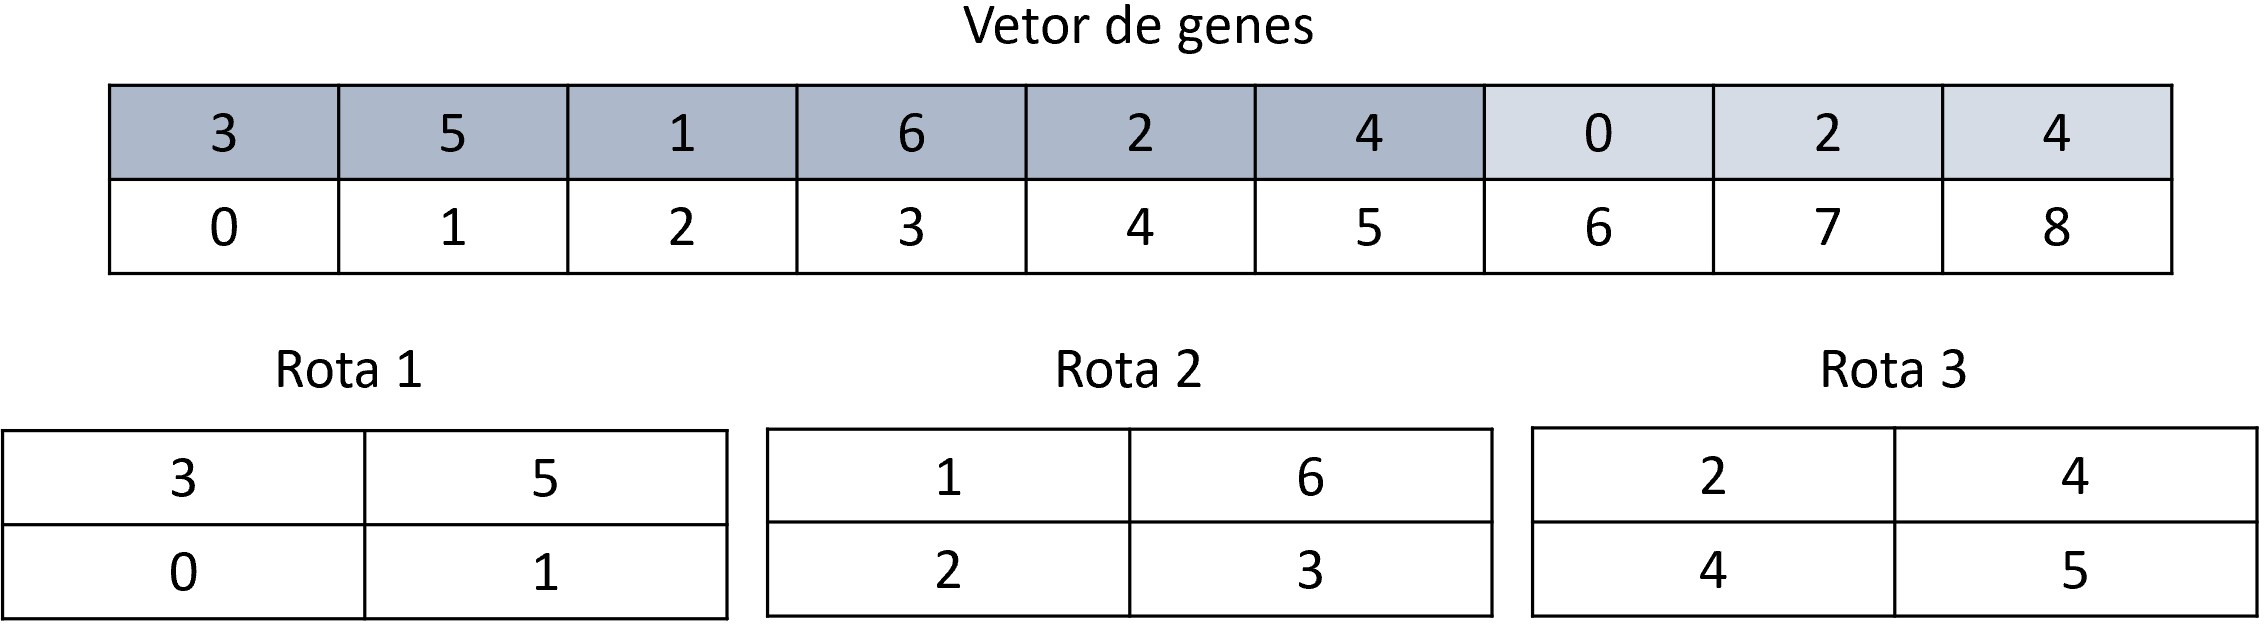
\includegraphics[width=.8\textwidth]{vrp_genes.jpg}
    \caption{Modelagem de um indiv\'{i}duo para o PRV}
    \label{fig:vrpGenes}
\end{figure}

Como visto na se\c{c}\~{a}o~\ref{sec:nonRepeating} \'{e} poss\'{i}vel utilizar uma estrutura de \textit{hash} para
acelerar o processo de busca de um elemento, mas ainda \'{e} necess\'{a}rio utilizar um vetor, porque o
\textit{hash} n\~{a}o \'{e} uma estrutura ordenada. Por\'{e}m para gerar a segunda parte deste vetor, \'{e} necess\'{a}rio que
os elementos gerados estejam em ordem crescente. Deste modo, ainda seria preciso executar um
algoritmo de ordena\c{c}\~{a}o ap\'{o}s a gera\c{c}\~{a}o dos elementos.

Para evitar esta etapa, uma solu\c{c}\~{a}o seria substituir o vetor por uma estrutura de \'{a}rvore ordenada. Existem
alguns tipos de \'{a}rvores ordenadas, e uma das mais utilizadas \'{e} a \'{a}rvore Rubro-Negra, devido \`{a} sua
capacidade de auto-balanceamento e garantia de busca de um elemento com complexidade $\mathcal{O}(\log_2n)$.
Assim \'{e} poss\'{i}vel armazenar os valores gerados em ordem enquanto s\~{a}o gerados.

Dependendo da quantidade m\'{a}xima de elementos deste vetor aleat\'{o}rio, utilizar somente uma \'{a}rvore pode
ser o suficiente para adquirir um desempenho aceit\'{a}vel. Mas ainda \'{e} poss\'{a}vel utilizar um \textit{hash}
auxiliar para acelerar verifica\c{c}\~{a}o de exist\^{e}ncia de um elemento. Assim a complexidade desta etapa seria
reduzida de $\mathcal{O}(\log_2n)$ para $\mathcal{O}(1)$.

\section{Implementa\c{c}\~{a}o}

Como existe uma grande quantidade de estruturas de dados existentes e cada uma possui pontos fortes e fracos,
\'{e} comum que se utilize em um projeto de software uma grande variedade delas, a fim de extrair a melhor utilidade
de cada uma. Entretanto, se fosse necess\'{a}rio implement\'{a}-las manualmente, o projeto se tornaria muito mais
demorado e talvez at\'{e} invi\'{a}vel. Al\'{e}m disso, muitas destas estruturas possuem implementa\c{c}\~{o}es
complexas e muitas vezes n\~{a}o se consegue alcan\c{c}ar o desempenho esperado com uma implementa\c{c}\~{a}o manual
porque \'{e} preciso muito tempo para refatorar o c\'{o}digo at\'{e} que ele alcance tal n\'{i}vel de efici\^{e}ncia.

Por estes motivos, \'{e} importante utilizar as estruturas de dados dispon\'{i}veis na biblioteca padr\~{a}o da linguagem
utilizada. O projeto da biblioteca padr\~{a}o \'{e} mais maduro e j\'{a} foi testado muitas vezes para garantir sua
efici\^{e}ncia, al\'{e}m de ser praticamente livre de \textit{bugs}. Todas as estruturas de dados citadas neste artigo
est\~{a}o dispon\'{i}veis na linguagem C++. Muitas delas tamb\'{e}m est\~{a}o dispon\'{i}veis em outras linguagens de
programa\c{c}\~{a}o, como Python e Java.

Mesmo que esta estrutura n\~{a}o esteja dispon\'{i}vel na linguagem de programa\c{c}\~{a}o desejada e n\~{a}o exista
uma solu\c{c}\~{a}o similar, pode-se optar por bibliotecas de terceiros que realizem esta implementa\c{c}\~{a}o. Apesar deste
m\'{e}todo n\~{a}o garantir um projeto eficiente e livre de \textit{bugs}, ainda \'{e} uma op\c{c}\~{a}o mais segura
do que realizar a implementa\c{c}\~{a}o manual.

Caso a pessoa esteja disposta a colaborar com o desenvolvimento de uma biblioteca de estrutura de dados, existem
diversos resposit\'{a}rios de c\'{o}digo aberto dispon\'{i}veis na internet. Assim, a pessoa tem a chance de
colaborar com uma equipe em um projeto que tem um potencial de ajudar muitos desenvolvedores.

\section{Conclus\~{a}o}

TODO

\section{Figures and Captions}\label{sec:figs}


Figure and table captions should be centered if less than one line
(Figure~\ref{fig:exampleFig1}), otherwise justified and indented by 0.8cm on
both margins, as shown in Figure~\ref{fig:exampleFig2}. The caption font must
be Helvetica, 10 point, boldface, with 6 points of space before and after each
caption.

\begin{figure}[ht]
\centering
\includegraphics[width=.5\textwidth]{fig1.jpg}
\caption{A typical figure}
\label{fig:exampleFig1}
\end{figure}

\begin{figure}[ht]
\centering
\includegraphics[width=.3\textwidth]{fig2.jpg}
\caption{This figure is an example of a figure caption taking more than one
  line and justified considering margins mentioned in Section~\ref{sec:figs}.}
\label{fig:exampleFig2}
\end{figure}

In tables, try to avoid the use of colored or shaded backgrounds, and avoid
thick, doubled, or unnecessary framing lines. When reporting empirical data,
do not use more decimal digits than warranted by their precision and
reproducibility. Table caption must be placed before the table (see Table 1)
and the font used must also be Helvetica, 10 point, boldface, with 6 points of
space before and after each caption.

\begin{table}[ht]
\centering
\caption{Variables to be considered on the evaluation of interaction
  techniques}
\label{tab:exTable1}
\includegraphics[width=.7\textwidth]{table.jpg}
\end{table}

\section{Images}

All images and illustrations should be in black-and-white, or gray tones,
excepting for the papers that will be electronically available (on CD-ROMs,
internet, etc.). The image resolution on paper should be about 600 dpi for
black-and-white images, and 150-300 dpi for grayscale images.  Do not include
images with excessive resolution, as they may take hours to print, without any
visible difference in the result. 

\section{References}

Bibliographic references must be unambiguous and uniform.  We recommend giving
the author names references in brackets, e.g. \cite{knuth:84},
\cite{boulic:91}, and \cite{smith:99}.

The references must be listed using 12 point font size, with 6 points of space
before each reference. The first line of each reference should not be
indented, while the subsequent should be indented by 0.5 cm.

\bibliographystyle{sbc}
\bibliography{sbc-template}

\end{document}
